\cleardoublepage
\chapter{Exploring some Testing Tools}
\minitoc

\section{Using the tools}\label{testingtools}
After introducing the theory and the techniques that support each tool, some of the tools will be demonstrated in action, resorting to small but illustrative examples
on how each tool can help us to find good test cases.\\

\subsection{PathCrawler}
Concerning the first case  a simple example will be used based on a function that performs a multiplication, creating a simple branch on the code.
\begin{code}[{Multiplication of a Point coordinates in C}]
typedef struct s {
    int x;
    int y;
}Point;

int Multiply(Point p) {
    if(p.x * p.y == 42) return 1;
    else return 0;
}
\end{code}
Pointers were tried instead of coping the structure as a parameter to $Multiply$ function, but PathCrawler was not able to run.

Nevertheless, PathCrawler was able to give a full coverage for this simple function as you can see in Table \ref{tab:mul}.

\begin{table}[!ht]
\renewcommand{\arraystretch}{1.3}
\setlength{\tabcolsep}{10pt}
\centering
\noindent \begin{tabular}{|c|c|c|}\hline
\textbf{Result} & \textbf{p} & \textbf{return value}\\\hline
\checkK & Point\{x=1,y=42\} & 1 \\\hline
\checkK & Point\{x=177407,y=109471\} & 0 \\\hline
\end{tabular}
\caption{Output Table for $Multiply$ function using PathCrawler}\label{tab:mul}
\end{table}

Regarding our second example a function that performs a binary search in order to find if a number is in a given range (between two bounds).

\begin{code}[{Binary Search in C}]
int BSearch(int x, int n) {
    return BinarySearch(x, 0, n); 
}
	
int BinarySearch(int x, int lo, int hi) {
    while (lo < hi) {
        int mid = (lo+hi)/2;
        pathcrawler_assert(mid >= lo && mid < hi);
        if (x < mid) { hi = mid; }
		else { lo = mid+1; }
    }
    return lo; 
}
\end{code}
A function that PathCrawler gives to us has been used: $pathcrawler\_assert$, this function can be used at any location in the
program under test, and will force PathCrawler to generate test cases to cover both the case where its argument is true and the case where it is false.
This feature may be seen as another way to write an oracle.\\
The results were interesting: 31 covered paths and 44 infeasible paths and the test was interrupted by PathCrawler,
because PathCrawler reach the maximal test session time (the user can increase this number, but for this example is left the default value).\\
A further analysis of the results demonstrated that 28 out of the 44 infeasible paths discovered appeared when PathCrawler tried to
do the assertion in line 8. No pre-condition was written, so PathCrawler does not know that this is a pre-condition
for $BinarySearch$ function:  $lo\leq~x<hi$. In Table \ref{tab:bsearch} is shown some of the test inputs generated for this example.

\begin{table}[!ht]
\renewcommand{\arraystretch}{1.3}
\centering
\noindent \begin{tabular}{|c|c|c|c|}\hline
\textbf{Result} & \textbf{x} & \textbf{n} & \textbf{return value} \\\hline
\checkK & -189424 & -140714 & 0 \\\hline
\checkK & 157819 & 0 & 0 \\\hline
\checkK & 1 & 1610612736 & 2 \\\hline
\checkK & 2 & 805306368 & 3 \\\hline
\checkK & 11 & 1610612736 & 12 \\\hline
\end{tabular}
\caption{Output Table for $BSearch$ function using PathCrawler} \label{tab:bsearch}
\end{table}

PathCrawler was tried with the following function that calculates the year of the $n^{th}$ day after 1980-01-01.

\begin{code}[{Predicate to verify if is a leap year in C}]
int IsLeapYear(int year) {
  return (year % 4 == 0) && ((year % 100 != 0) || (year % 400 == 0));
}
int FromDayToYear(int day) {
  int year = 1980;

  while (day > 365) {
    if (IsLeapYear(year)) {
      if (day > 366) {
        day -= 366;
        year += 1;
      }
    } else {
      day -= 365;
      year += 1;
    }
  }
  return year;
}
\end{code}

The result was unexpectedly $unknown$. PathCrawler was unable to trace even one path in our code, the number of $k$-path's could
be increased but with no success for this example.

\subsection{Pex}
Regarding Pex, we used the same examples shown previously adapted to C\# language.
Because C\# is a more expressive language than C our examples will be improved with some other \ac{OO} and C\# specific features like Exceptions and Debug.Assert calls.
In fact Pex can also support a lot more features that are present in C\# language like .NET Contracts and many more.\\
This is the simple implementation of a 2D $Point$ class that has been created to have special behavior, under a certain condition
$x \times y \equiv 42$ it is supposed to throw an exception.

\begin{code}[{Multiplication of a Point coordinates in C\#}]
\begin{code}
public class Point {
  public readonly int X, Y;
  public Point(int x, int y) { X = x; Y = y; }
}

public class Multiply {
  public static void multiply(Point p) {
    if (p.X * p.Y == 42)
        throw new Exception("hidden bug!");
  }
}
\end{code}

So, as was described earlier, Pex will try to generate such input as it is possible (in a given amount of time) to traverse all the paths inside the code.
The output table can be seen in Table \ref{tab:point}, with the inputs and outputs that Pex found to ensure a full coverage of the code.

\begin{table}[!ht]
\renewcommand{\arraystretch}{1.3}
\setlength{\tabcolsep}{1pt}
\centering
\noindent \begin{tabular}{|c|c|c|c|}\hline
\textbf{Result} & \textbf{p} & \textbf{Output/Exception} & \textbf{Error Message}\\\hline
 &  &  & Object ref. not set \\
\cross & null  & NullReferenceException & to an instance \\
 &  &  & of an object.\\\hline
\checkK & new Point\{X=0,Y=0\} & &\\\hline
\cross & new Point\{X=3,Y=14\} & Exception & hidden bug!\\\hline
\end{tabular}
\caption{Output Table for $multiply$ method using Pex}\label{tab:point}
\end{table}

Pex was successful to reach the $Exception$ path inside the code. Of course this is not always possible, since sometimes the functions inside
the $if$ statement does not have inverse function.\\

Pex can also be very helpful checking assertions and contracts in .net code. A binary search algorithm was written and an assertion was also written in
the middle of our code.

\begin{code}[{Binary Search in C\#}]
public class Program {
  public static int BSearch(int x, int n) {
    return BinarySearch(x, 0, n);
  }
  static int BinarySearch(int x, int lo, int hi) {
    while (lo < hi) {
      int mid = (lo+hi)/2;
      Debug.Assert(mid >= lo && mid < hi);
      if (x < mid) { hi = mid; } else { lo = mid+1; }
    }
    return lo;
  }
}
\end{code}

Pex was able to generate an input that could not pass in the assertion inerted in our code, as can be seen in Table \ref{tab:binary}.

\begin{table}[!ht]
\renewcommand{\arraystretch}{1.3}
\setlength{\tabcolsep}{1pt}
\centering
\noindent \begin{tabular}{|c|c|c|c|c|}\hline
\textbf{Result} & \textbf{x} & \textbf{n} & \textbf{result} & \textbf{Output/Exception}\\\hline
\checkK & 0 & 0 & 0      & \\\hline
\checkK & 0 & 1 & 1      & \\\hline
\checkK & 0 & 3 & 1      & \\\hline
\cross & 1073741888 & 1719676992 & & TraceAssertionException \\\hline
\checkK & 1 & 6 & 2      & \\\hline
\checkK & 50 & 96 & 51      &\\\hline
\end{tabular}
\caption{Output Table for $BSearch$ method using Pex}\label{tab:binary}
\end{table}

Now we have a more complex example, a function that returns the year of the $n^{th}$ day after 1980-01-01.
Pex was able to generate some important test cases, but it has reached the limit amount of time to calculate interesting paths in the code,
this boundary prevents Pex from getting stuck when the program goes into
an infinite loop.

\begin{code}[{Predicate to verify if is a leap year in C\#}]
public class Program {
  private static bool IsLeapYear(int year) {
    return (year % 4 == 0) && ((year % 100 != 0) || (year % 400 == 0));
  }
  public static void FromDayToYear(int day, out int year) {
    year = 1980;
    while (day > 365) {
      if (IsLeapYear(year)) {
        if (day > 366) {
          day -= 366;
          year += 1;
        }
      } else {
        day -= 365;
        year += 1;
      }
    }
  }
}
\end{code}

Pex was unable to discover the year for day $366$ and $7671$ as we can see in Table \ref{tab:leap}.
This problem occurred because Pex by default has a maximum number of conditions, this avoids never ending functions and still has a result from Pex.
In this particular case we could increment the number of $MaxConditions$: $[PexMethod(MaxConditions=10000)]$.

\begin{table}[!ht]
\renewcommand{\arraystretch}{1.3}
\centering
\noindent \begin{tabular}{|c|c|c|c|c|}\hline
\textbf{Result} & \textbf{day} & \textbf{out year} & \textbf{Output/Exception}\\\hline
\checkK & 0 & 1980 & \\\hline
\checkK & 367 & 1981 & \\\hline
\bigexclaim & 366 & & path bounds exceeded\\\hline
\checkK & 1023 & 1982 &\\\hline
\checkK & 2561 & 1987 & \\\hline
\checkK & 7874 & 2001 & \\\hline
\bigexclaim &  7671 & & path bounds exceeded\\\hline
\end{tabular}
\caption{Output Table for $FromDayToYear$ method using Pex}\label{tab:leap}
\end{table}

\subsection{Korat}
Like was explained before, Korat generates a graphical representation of the structure instances that validates the property $repOK$. This property was written using JAVA code.\\
In order to test the freelly available version of Korat, a Doubly Linked List structure was created in JAVA.

\begin{code}[{LinkedList class in JAVA}]
public class LinkedList<T> {
  public static class LinkedListElement<T> {
    public T Data;
    public LinkedListElement<T> Prev;
    public LinkedListElement<T> Next;
  }
  private LinkedListElement<T> Head;
  private LinkedListElement<T> Tail;
  private int size; 
}
\end{code}

\def\t#1#2#3#4{\langle#1 \ #2 : #3 \ : #4 \ \rangle}
\def\d#1#2#3{\langle#1 \ #2 :: #3 \ \rangle}
\newcommand{\subseteqL}{\mathbin{\subseteq\mkern-4mu\subseteq}}
\newcommand{\inL}{\mathbin{\in\mkern-4mu\in}}

Now the $repOK$ predicate method must be defined.
This predicate method will check that the tree doesn't have any cycles and that the number of nodes traversed from root matches the value of the field size.
First was defined the properties about this data structure. The most relevant ones are property \ref{eq:linked} in Figure \ref{fig:formulae} that
ensures the structure and property \ref{eq:uniq} that ensures our doubly linked list does not have repeated elements.\\
Consider $e,e_1,e_2 \in LinkedListElement$ and $i$ the index function: $i : LinkedListElement \rightarrow int$, that receives an element of $LinkedList$ and
returns the position of that element in the structure. Consider also three new functions:
\begin{enumerate}
\item $Head(l)$ being $l$ of type $LinkedList$ and meaning in Java code $l.Head$.
\item $Tail(l)$ being $l$ of type $LinkedList$ and meaning in Java code $l.Tail$.
\item $size(l)$ being $l$ of type $LinkedList$ and meaning in Java code $l.size$.
\end{enumerate}

As a matter of avoiding verbosity two symbols were defined ($\inL$ and $\subseteqL$, these symbols are used to define the $LinkedList$ invariants in Figure \ref{fig:formulae}):
\begin{enumerate}
\item $a \inL l$ being $a$ of type $LinkedListElement$ and meaning that $a$ is an element of the $LinkedList$ $l$.
\item $\{a,\ldots,z\} \subseteqL l$ meaning $a \inL l \wedge \ldots \wedge z \inL l$.
\end{enumerate}

\begin{figure*}[!Hb]
\begin{eqnarray}
\t \forall {l} {l \in LinkedList} {Head(l) \equiv null \vee Tail(l) \equiv null \Leftrightarrow size(l) \equiv 0}\\
\t \forall {l} {l \in LinkedList} {Tail(l).Next \equiv null}\\
\t \forall {l} {l \in LinkedList} {Head(l).Prev \equiv null}\\
\t \forall {l} {l \in LinkedList} {size(l) \equiv 1 \Leftrightarrow Head(l) \equiv Tail(l)}\\
\t \forall {l} {l \in LinkedList} {\t \forall {e_1,e_2} {\{e_1,e_2\} \subseteqL l} {\t \exists {e} {e \inL l} {e_1.Next \equiv e \wedge e_2.Prev \equiv e}}\label{eq:linked}}\\
\t \forall {l} {l \in LinkedList} {\t \forall {e_1,e_2} {\{e_1,e_2\} \subseteqL l} {e_1 \equiv e_2 \Rightarrow i(e_1) \equiv i(e_2)}\label{eq:uniq}}
\end{eqnarray}
\caption{Invariants for class $LinkedList$}
\label{fig:formulae}
\end{figure*}

We took the properties described in Figure \ref{fig:formulae} and use them to restrict the generation of structures as we can see in the following Java implementation code.
Note that we using short-circuiting, so we return $false$ as soon as we can. This way Korat will be able to generate faster the instances matching our criteria.

\begin{code}[{repOK Korat method for LinkedList class in JAVA}]
public boolean repOK() {
  if(Head == null || Tail == null)
    return size == 0;
  if(size == 1) return Head == Tail;
  if(Head.Prev != null) return false;
  if(Tail.Next != null) return false;
  LinkedListElement<T> last = Head;
  Set visited = new HashSet();
  LinkedList workList = new LinkedList();
  visited.add(Head);
  workList.add(Head);
  while (!workList.isEmpty()) {
    LinkedListElement<T> current = (LinkedListElement<T>) workList.removeFirst();
    if (current.Next != null) {
      if (!visited.add(current.Next))
	    return false;
      workList.add(current.Next);
      if(current.Next.Prev != current) return false;
      last = current.Next;
    }
  }
  if(last != Tail)
    return false;
  return (visited.size() == size);
}
\end{code}

The last step was defining the finitization method, this way we tell Korat how to bound the input space.

\begin{code}[{Finitization Korat method for LinkedList class in JAVA}]
public static IFinitization finLL(int nodesNum, int minSize, int maxSize) {
  IFinitization f = FinitizationFactory.create(LL.class);
  IObjSet nodes = f.createObjSet(LinkedListElement.class, nodesNum, true);
  f.set("Head", nodes);
  f.set("Tail", nodes);
  f.set("size", f.createIntSet(minSize, maxSize));
  f.set("LinkedListElement.Next", nodes);
  f.set("LinkedListElement.Prev", nodes);
  return f;
}
\end{code}

The properties in Figure \ref{fig:formulae} were taken and used to restrict the generation of structures using Java. So the $repOK$ method that receives
a $LinkedList$ structure and returns $Bool$ whenever this structure follows the invariants in \ref{fig:formulae} was defined.
Using this specification, Korat generated the 2 structures shown in Figure \ref{fig:inst1} and \ref{fig:inst2}. In Figure \ref{fig:inst1} with $2$ elements
and in Figure \ref{fig:inst2} an instance with $5$ elements.

\begin{figure}[!ht]
\centerline{
\subfloat[Instance with $2$ elements for $LinkedList$]{
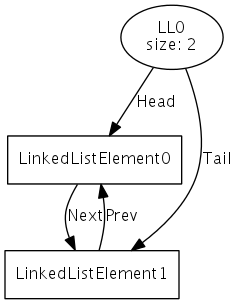
\includegraphics[width=.3\textwidth]{images/ll1}
\label{fig:inst1}
}
\hfil
\subfloat[Instance with $5$ elements for $LinkedList$]{
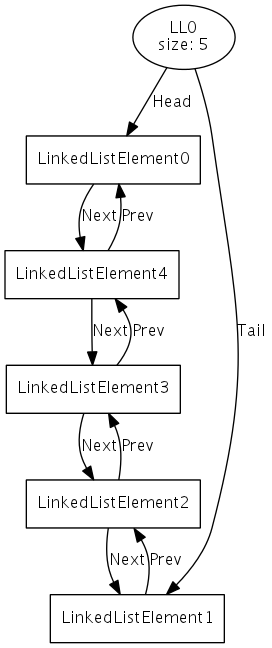
\includegraphics[width=.25\textwidth]{images/ll2}
\label{fig:inst2}}}
\caption{Examples of generated instances from Korat for $LinkedList$ class.}
\label{fig:insts}
\end{figure}

\subsection{Summary}
After the experimental study of the selected tools, reported in the previous subsections, it was found that PathCrawler and Pex have different
approaches regarding testcase generation. PathCrawler seems to be a very efficient tool to discover multiple
infeasible paths in C code, because it uses a mix between static and dynamic analysis. When it finds a suitable input for a function it tries to execute
collecting all the executed paths in the code.
Pex on the other side just uses static execution and it is very efficient discovering all the feasible paths in C\# methods. Pex was also used
to perform testcase generation in C\# classes, but the generated instances are too simple to perform more interesting tests. The $LinkedList$ class was written
in C\# with many management methods implemented (Add, Remove, Find,\ldots). Pex generated very simple $LinkedList$'s structures to perform automatic test generation
for each implemented method. The problem is that the generated structures does not meet the properties about Doubly Linked Lists as it can be seen in Figures \ref{fig:pexinst1} and \ref{fig:pexinst2}.
Concerning Korat, this is The tool to generate complex data structures. The freely available part of Korat show potential in expressing rules to hedge
the automatic generation of data structures.\\
In Table \ref{tab:tabcmp} we can see a brief comparison between all the experimented and mentioned tools, a more detailed conclusion is addressed in Chapter \ref{Concl}.

\begin{table}[!ht]
\centering
\begin{tabular}{|m{2.5cm}|m{1cm}|m{2cm}|m{2cm}|m{3.5cm}|m{3.5cm}|}\hline
\textbf{Name} & \textbf{Target Language} & \textbf{Type} & \textbf{Additional Input} & \textbf{Output} & \textbf{Comments}\\\hline
\textbf{PathCrawler} & C & White-box (symbolic execution) & Test vectors & Constraints about the executed paths & Too Complex\\\hline
\textbf{Pex} & C\# & White-box (symbolic execution) & -- & Unit Tests & Poor generated data instances (objects)\\\hline
\textbf{Korat} & JAVA & Black-box & Invariants written in JAVA & Graphical form of data structures (using Alloy-GraphViz) & Powerful generating valid data instances\\\hline
\end{tabular}
\caption{Comparison of experimented and mentioned tools}
\label{tab:tabcmp}
\end{table}

\begin{figure}[!ht]
\centerline{
\subfloat[Example of Pex generated $LinkedList$ instance to test $Remove$ method]{
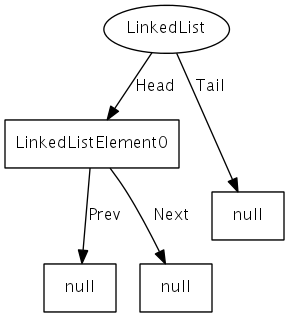
\includegraphics[width=.25\textwidth]{images/pex1}\label{fig:pexinst1}
}
\hfil
\subfloat[Example of Pex generated $LinkedList$ instance to test $Find$ method]{
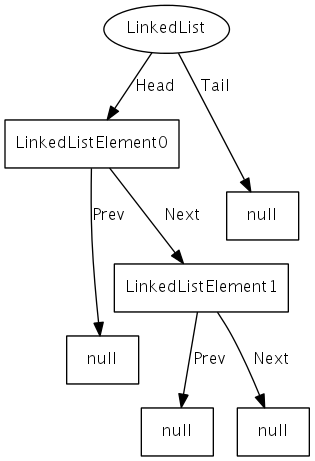
\includegraphics[width=.25\textwidth]{images/pex2}\label{fig:pexinst2}}}
\caption{Examples of generated instances from Pex for $LinkedList$ class.}\label{fig:pexG}
\end{figure}

%\section{Conclusion}\label{Concl}
%Looking for an efficient solution to automatically generate complete test sets for complex and critical C++ software,
%the state-of-the-art approaches in the area were studied and along the document some tools were introduced from methodological and experimental perspectives.
%Pex has proved to be a very powerful tool, aimed at offering a full coverage. However, the incapability for generating calling-methods sequences was a bit disappointing. 
%With Microsoft's SpecExplorer we can already
%manually call sequences of methods; maybe a combination of this feature with Pex would make Pex a perfect all-in-one testing tool regarding .NET automatic testing tools.
%Concerning Korat, the expected improvement is just to write the invariants for a class instead of the $repOK$ method, or maybe infer these invariants 
%from the existing code. Writing the $repOK$ method for very complex data structures requires some previous experience with Korat, but we think
%this is not a weakness, since the tester quickly gets used to write the $repOK$ method in Korat. The only problem is that right now we can not fully automate the process
%without human help.\\
%\indent Considering the studied tools and thinking about a full automated test generation tool, a clever composition among between Pex to ensure the maximum possible coverage, 
%Korat to generate all the valid data structures and an automatic tool to generate calls to methods combinations would be the perfect tool.\\
%
%At the end, it was proposed  an approach based on the inference of tests from a Code+OCL.
%\indent Concerning the OCL inference from C++ code, work will now be done on a tool that implements it.
%For that purpose, Frama-C will be explored, as it is well known that this tool is able to infer pre- and post-conditions\cite{moy}
%and interesting safety conditions from C source code.

\secendnote
